\section{Detektor}\label{sec:detect}
Feature detektion er en metode indenfor billedbehandling, der for hvert punkt $p = (x,y)$ i et billede $I$ bestemmer, om punktet er et interessepunkt. Denne kan beskrives ved:
\begin{equation}
Detect(I)= \bold{P}
\label{detect}
\end{equation}
hvor $\bold{P} = {p_1, p_2,..., p_n}$ er et sæt punkter i billedet $I$ udvalgt til at være interessepunkter. Moravec \cite{moravec} definerer, som en af de første, et interessepunkt(feature) således: "A
feature is good if it can be located unambiguously in different views of a scene. A
uniformly colored region or a simple edge does not make for good features because
its parts are indistinguishable". Iflg. Moravec skal et interessepunkt have egenskaber der gør det utvetydigt lokaliserbart. Denne definition, sammen med Lindebergs \cite{pointsurvey} er her blevet adopteret, og et interessepunkt karakteriseres her ved:
\begin{itemize}
\item{\emph{Repeterbar}: Repeterbarheden significere uafhængighed af forskellige betingelser i billedet. Dvs. at samme interessepunkt skal kunne findes i to forskellige billeder, trods ændringer af f.eks lys og rotation}
\item{\emph{Informationsrigt:}
Intensiteten i og omkring interessepunktet skal være unikt, da dette muliggør en mere detaljeret beskrivelse af punktet. Et punkt placeret på et område af samme intensitet, vil ikke kunne skelnes fra andre punkter placeret i samme i område..}
\item{\textit{Definerbar struktur:} Punktet skal indgå i en struktur, der er matematisk definerbar. Dette er nødvendigt da punkterne skal kunne identificeres uafhængigt i begge billeder.}
\end{itemize}
\raggedbottom\subsection{Skalarum}
\label{sec:scale}
Objekter i virkeligheden, såvel som afbilledet, optræder forskelligt, alt efter hvilken afstand de observeres fra. Et træ vil indenfor centimeters eller nanometers afstand, optræde som blade eller molekyler og indenfor meters afstand, som et træ. Ved skalaforskelle imellem billeder af samme scene ønskes det at objekter, indgående i scenen, kan sammenlignes på trods af skalaforskellene. Problemet er at skalaændringen ikke kendes. En tilgang til dette problem er at repræsentere billedet på flere forskellige skalaer. Dette kan udføres i form af en udvidelse af billedfunktionen fra ligning \eqref{bf}, med en enkelt parameter, også kaldt skalaparametren $\sigma$:
\begin{equation}
\begin{split}
&L: \mathbb{R}^3 \rightarrow \mathbb{R} \\
&L(x,y,\sigma) = \lambda_{x,y} \hspace{0.5 cm} (x,y,\sigma)\in \mathbb{R}^3, \lambda_{x,y} \in [1,256] \subset \mathbb{R}
\end{split}
\end{equation}
% Bekræft søren
For at opnå en multi-skala repræsentation af billedet, oprettes der et skalarum bestående af en stak skalabilleder, der går fra at udtrykke finere til grovere strukturer, proportionelt med skalaparametren, som illustreret i figur \ref{fig:scalerep}. 
\begin{figure}[H]
    \centering
    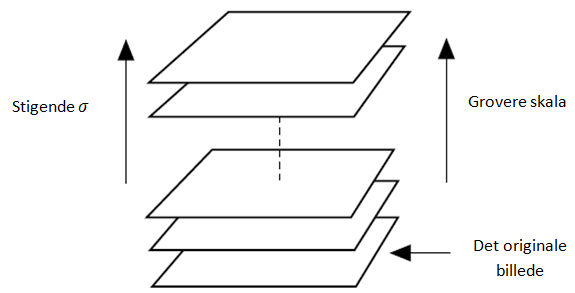
\includegraphics[width=0.55\textwidth]{fig/32.png}
     \vspace{-0.5em}
    \begin{center}    
       \caption{{\footnotesize \textit{En lineær skalarums repræsentation af et billede. Skalabillederne opstilles som en stak af billeder udsat for stigende grad af slørring}}}
    \label{fig:scalerep}
     \end{center}
     \vspace{-2.5em}
  \end{figure} \noindent
Denne overgang fra finere til grovere strukturer kan opnås ved systematisk at folde et billede med et Gaussisk filter af stigende sigmaværdi, hvor det nederste billede i stakken kan repræsenteres ved billedet $ L(x,y,0) = I(x,y)$ og for $\sigma>0$, defineres et skalabillede ved:
\begin{equation}
L(x,y,\sigma) = G(x,y,\sigma)\ast I(x,y)
\label{scalespace1}
\end{equation}
\\
Filteret der bruges til at oprette en skalarumsrepræsentation, skal opfylde følgende egenskaber:
\begin{itemize}
\item{Et lokalt ekstrema må ikke forøges når skalaparametren stiger. Dette medfører at støj i billedet ikke tilføjes, når skalaparametren stiger \cite{lindkth}.}
\item{Hvis hver udglatnings kerne er tilknyttet en skalaparameter, og to kerner foldes med hinanden, ønskes det at den resulterende kerne har en skalaparameter, lig med summen af de foregående skalaparametre \cite{springer}.
\begin{equation}
g(\cdot;\sigma_1) \ast g(\cdot;\sigma_2)=g(\cdot;\sigma_1+\sigma_2)
\label{semi}
\end{equation}
Ovenstående viser at alle skalarums transformationer er af samme familie. En skalarums repræsentation ved en grov skala $\sigma_2$, kan derved udledes, ved en repræsentation fra en finere skala:
\begin{equation}
g(\cdot;\sigma_2) = g(\cdot;\sigma_2-\sigma_1)\ast g(;\sigma_1)\text{,}\sigma_2>\sigma_1
\end{equation}}
\end{itemize}
Der anvendes et Gaussisk filter da den imødekommer begge ovenstående egenskaber. Ved et Gaussisk filter vil strukturer, der eksistere på grovere skalaer være simplificeringer af strukturer fra finere skalaer. Witkin \cite{witkins} beviste dette i tilfældet for én-dimensionsalle signaler illustreret i figur \ref{scalespace1}, der viser resultatet af at glatte et signal med et Gaussisk filter af stigende sigmaværdi. Det ses tydeligt, hvordan signalets underliggende grovere struktur bliver udtrykt og at finere strukturer undertrykkes.
\begin{figure}[H]
    \centering
    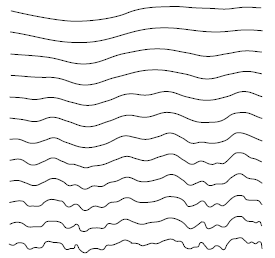
\includegraphics[width=0.45\textwidth]{fig/33.png}
     \vspace{-1em}
    \begin{center}    
       \caption{{\footnotesize \textit{Et én-dimensionalt signal udsat for et Gaussisk filter af gradvist stigende størrelse.}}}
    \label{fig:scalereps}
     \end{center}
     \vspace{-2.5em}
  \end{figure} \noindent
\subsubsection*{Skala Pyramide}
En udbredt metode, hvorpå skalarummet kan repræsenteres, er ved en \textit{skalapyramide}. Ved en skalapyramide repræsentation oprettes en pyramide af kopier af det undersøgte billede, hvor der for hvert niveau i pyramiden sker en reduktion af billedets størrelse, med en faktor af to. 
Når billedets størrelse skal halveres, er det ikke nok bare at fjerne hver anden række og hver anden kolonne, da dette vil resultere i store tab af billedets informationer. For at imødekomme dette problem, foldes billedet med et Gaussisk filter, inden billedet reduceres.  
Hvert niveau i pyramiden kaldes en oktav. Sigmaværdien fordobles imellem hver oktav.
 \begin{figure}[H]
    \centering
    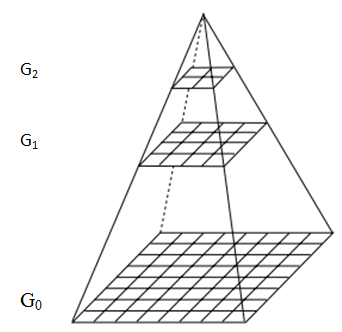
\includegraphics[width=0.40\textwidth]{fig/40.png}
     \vspace{-1em}
    \begin{center}    
       \caption{{\footnotesize \textit{En pyramiderepræsentation af et billede, der reduceres med en faktor af to, for hvert niveau. }}}
    \label{fig:scalerepdiff}
     \end{center}
     \vspace{-2.5em}
  \end{figure} \noindent
Hvis $G_0=I(x,y)$, kan de forskellige niveauer $l$ i skalapyramiden opnås ved:
\begin{equation}
G_l(i,j)=\sum\limits_{m}\sum\limits_{n}w(m,n)G_{l-1}(2i+m,2j+n)
\end{equation}
hvor $w$ er et Gaussisk filter. Fordelene ved en pyramiderepræsentation er at billedernes størrelser reduceres, hvilket reducere antallet af beregninger drastisk.
\raggedbottom\subsection{Strukturer}
Der findes mange definitioner af et interessepunkt, og i sidste ende angiver anvendelsesområdet, hvilke punkter, der lokaliseres bedst.
Interessepunkter defineres ikke udefra semantisk meningsfulde områder, som ansigter eller bøger, da dette vil kræve en høj-niveau fortolkning af scenen. I stedet anvendes lav-niveau strukturere, der identificeres i lokale pixelområder, der er matematisk definerbare. Nedenstående er en gennemgang af forskellige lokale lav-niveau strukturere, der kan bruges i udvælgelsen af interessepunkter.
\subsection{Hjørner}\label{subsec:corner}
At detektere hjørner er en udbredt teknik indenfor feature detektion, da hjørner ofte forekommer i forskellige menneskeskabte scener og fordelagtigt kan bruges i disse sammenhæng. Et hjørne kan defineres som et område i og omkring et punkt, der har to dominerede kantretninger og kan derved lokaliseres i et billede udefra en kvantificeret fortolkning af dette. \\ Udover at være lokaliserbare ved en matematisk definition, skal et interessepunkt besidde en unik struktur, der tillader en entydig korrespondance. I figur \ref{app} ses tre udvalgte punkter, placeret forskelligt i samme scene, hvor punkterne beskrives af en blå cirkel omkring punktet. Figuren illustrere mulige korresponderende punkter, for et givent interessepunkt.
\begin{enumerate}[label=\alph*]
\item{Interessepunktet er placeret på et fladt området, hvor intensiteten er ens for hele området. Punktet vil have mange mulige korresponderende punkter.}
\item{ Interessepunktet er lokaliseret på en kant. Punktet vil have flere mulige korresponderende punkter på den tilsvarende kant i den anden figur.}
\item{Interessepunktet er lokaliseret på et hjørne. Det ses at kun ét andet punkt i modsvarende scene er identisk med dette.}
\end{enumerate}
\begin{figure}[H]
    \centering
    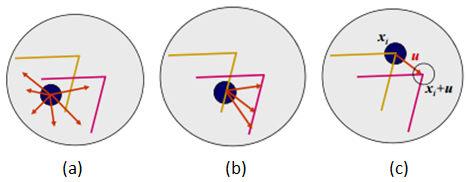
\includegraphics[width=0.55\textwidth]{fig/37.png}
    \vspace{-1em}   
    \begin{center}    
    \caption{\textcolor{gray}{\footnotesize \textit{
 }}}
    \label{app}
     \end{center}
    \vspace{-2.7em}  
  \end{figure}  
\noindent
Ovenstående definition viser at punkter placeret på hjørner er unikke og kan derfor entydigt differentieres fra ikke korresponderende punkter. Hjørner kan som nævnt udvælges i billederne pga. de dominerende kantretninger i og omkring punktet, hvilket medfører store intensitetsskift i området omkring et hjørne. En af de første hjørne detektorer udviklet af Moravec \cite{Moravec} lokalisere et hjørne ved at estimere auto-korrelationen imellem regioner af billedet, og definere hjørner, hvor der forekommer store intensitetsskift omkring et punkt.
\subsection{Blobs}
En blob er en region i et billede, hvor intensitet er konstant, og forskellig fra intensiteten udenfor regionen. Lindenberg \cite{blob} definere blobs som værende lyse regioner på sort baggrund eller omvendt - altså strukturer, der står i kontrast til deres baggrund. 

%Det lokale ekstrema gør blobben til en veldefineret, lav-niveau struktur og kravet om konstant intensitet gør den pr. definition distinktiv. 
\begin{figure}[H]
    \centering
    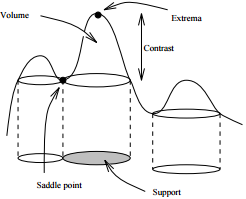
\includegraphics[width=0.35\textwidth]{fig/11.png}
    \vspace{-0.5em}   
    \begin{center}
    \caption{\textcolor{gray}{\footnotesize \textit{
    En blob visualiseret i 2-d, udefra Lindenberg's definition \cite{blob}}}}
    \label{fig:lindblob}
     \end{center}
  \end{figure}
       \vspace{-2.7em}
\noindent
%MEGA FORKERT
%MEGA FORKERT
%MEGA FORKERT
%MEGA FORKERT
I figur \ref{fig:lindblob}(a), ses en blob defineret af dens lokale ekstrema, hvor styrken af blobben beksrives ved kontrasten, ift. området omkring ekstremaet. Lindenberg definere en blob som værende afgrænset af dens saddelpunkt; et saddelpunkt angiver punktet, hvor intensiteten stopper med at falde og starter med at stige for lyse blobs, og modsat for mørke.
%MEGA FORKERT
%MEGA FORKERT
%MEGA FORKERT
%MEGA FORKERT
%MEGA FORKERT
%MEGA FORKERT
%MEGA FORKERT
\\
\\
En metode til at detektere ekstremaer, er Laplace af Gauss(LoG). Laplace defineres således:
\begin{equation}
\Delta f = \nabla^2 f =  \sum_{i = 1}^n \frac{\partial^2 f}{\partial x^2_i}
\end{equation}
Anvendes Laplace operatoren på Gaussfunktionen (ligning \eqref{2dgaussian}), kan resultatet diskretiseres og anvendes som en kerne.
\begin{equation}
LoG= \sigma^2\Delta G
\label{lap}
\end{equation}
Bemærk, at $\sigma^2$ er blevet multipliceret på fra venstre. Dette er gjort for at normalisere LoG, således, at responset er invariant overfor størrelsen af $\sigma$. LoG kan diskritiseres og foldes med billedet for at finde lokale ekstremaer. \\

\begin{figure}[H]
    \centering
    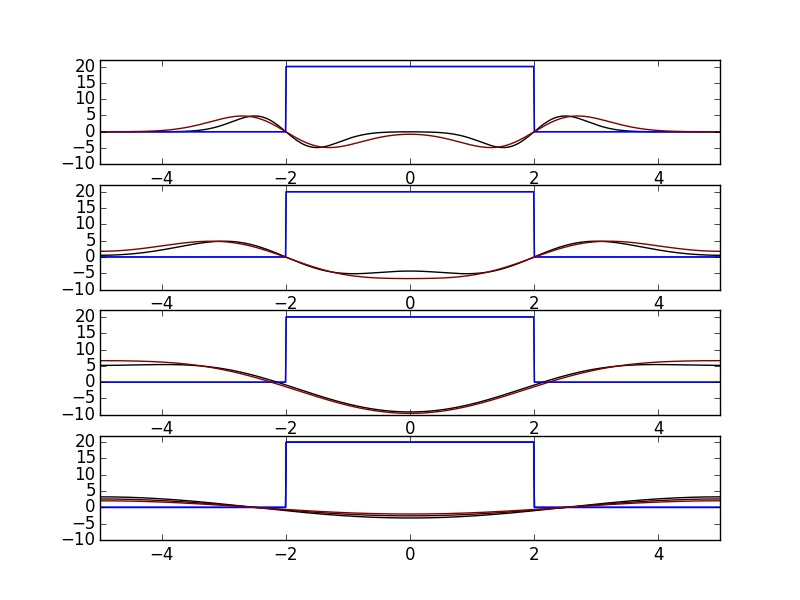
\includegraphics[width=0.90\textwidth]{fig/normLoG.jpg}
    \vspace{-0.5em}   
    \begin{center}
    \caption{\textcolor{gray}{\footnotesize \textit{
    (a) En 3-D visualisering af en to-dimensional Laplacian of Guassian (b) ét en-dimensionalt signal (c) Laplacian of Gaussian operatoren anvendt på (b)}}}
    \label{fig:normLoG}
     \end{center}
  \end{figure}
       \vspace{-2.5em}
\noindent
Når blobs skal lokaliseres, skal $\sigma$ værdien være tilpasses blobbens størrelse, som ses på figur \eqref{fig:normLoG}. Figuren viser fire forskellige værdier for $\sigma$. I første illustration er $\sigma$ værdien for lav - her dannes flere ekstremaer, men ingen af dem karakteriserer en blob, da den absolutte værdi for funktionen evalueret på det afledte af LoG signalet, er for lav. Dog ser kurven i illustration tre ud til, at have tilstrækkelig høj absolut værdi, til at kunne karakteriseres som et blob. \\
Problemet omkring valg af skala, kan afhjælpes ved skalarumsrepræsentation, som gennemgås i.

\begin{figure}[H]
    \centering
    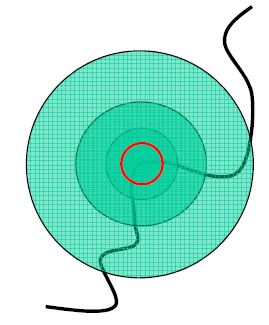
\includegraphics[width=0.25\textwidth]{fig/29.png}
    \vspace{-0.5em}   
    \begin{center}
    \caption{\textcolor{gray}{\footnotesize \textit{
    }}}
    \label{fig:scale}
     \end{center}
  \end{figure}
       \vspace{-2.5em}
\noindent
I figur \ref{fig:scale} angiver cirklerne forskellige undersøgte skalaer, Så hvordan udvælges cirklen, der dækker interesse området uafhængigt af områdets størrelse?  For Blobs er det interessant når der i et skaleret område opstår et veldefineret ekstrema. En måde at søge efter ekstremaer over forskellige skalaer er ved at oprette et skalarum for det undersøgte billede, hvor hvert billede skaleres og der for hver skala findes interessepunkter. Skala-rummet i et 2-dimensionalt billede repræsenteres af flere billeder i forskellige skalaer af det originale billede. Billeder, der repræsentere forskellige skalaer, opnås ved at folde billedet iterativt med et Gaussisk filter med stigende $\sigma$ værdi. 
\begin{figure}[H]
    \centering
    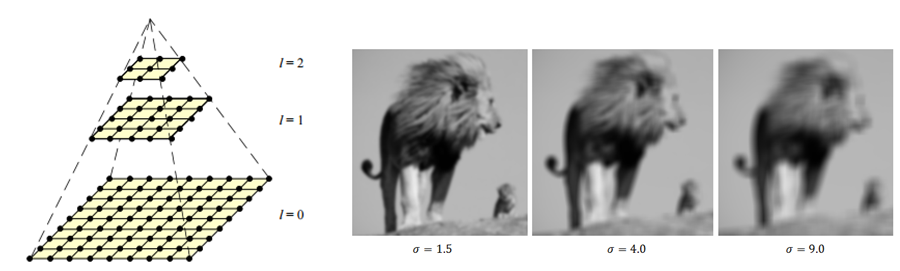
\includegraphics[width=0.65\textwidth]{fig/24.png}
    \vspace{-0.5em}   
    \begin{center}
    \caption{\textcolor{gray}{\footnotesize \textit{
Til venstre ses en visualisering af et skala-rum formet som en pyramide. Hvert niveau angiver en skala repræsentation af det originale vindue, hvor toppen af pyramiden indeholder billeder af største skala og derfor med mindst information, og bunden af skalaen med det originale billede. Til højre ses et billede foldet med et Gaussisk filter af stigende sigma værdier. Jo højere sigma værdi, jo flere fine detaljer bliver fjerne og billedet slørret.
    }}}
    \label{fig:mona}
     \end{center}
  \end{figure}
       \vspace{-2.5em}
\noindent
Et Gaussisk filter bruges da gradvis højere værdier af $\sigma$ fjerner fine strukturer, som vist i figur \ref{fig:mona}, og nye strukturer forekommer ikke ved transformationen fra finere til grovere skalaer \cite{lindenscale}. Idéen er derved at fjerne disse strukturer og lede efter  andre ekstremaer, gradvist på større skalaer, der også kan detekteres.
Et billede i skalarummet for billedet $f(x,y)$ kan derfor defineres som i \eqref{scalespace}
\begin{equation}
L(x,y,\sigma) = G(x,y,\sigma)\ast f(x,y)
\label{scalespace}
\end{equation}
hvor $G$ er det 2-dimensionelle Gaussiske filter,$L(x,y,\sigma)$ repræsentere et et billede i skala-rummet, og skala-parametren $\sigma$, bestemmer skalaen, eller placeringen i skala-rummet. $L(x,y,0) = f(x,y)$, da det er den "nederste" skala og den nederste del af pyramiden. Højere niveauer af pyramiden kan opnås ved at folde billedet med et Gaussisk filter af større sigma værdi.